\documentclass{article}

% content/resources/templates/preamble.tex
\usepackage[margin=0.6in]{geometry}
\author{Milav Dabgar}
\usepackage{amsmath,amssymb,amsthm}
\usepackage{booktabs}
\usepackage{multirow}
\usepackage{xcolor}
\usepackage{tcolorbox}
\tcbuselibrary{breakable,skins}
\usepackage[colorlinks=true,linkcolor=blue]{hyperref}
\usepackage{titlesec}
\usepackage{enumitem}
\usepackage{tikz}
\usepackage{pgfplots}
\usepackage{circuitikz}
\usepackage[version=4]{mhchem}
\usepackage{longtable}
\usepackage{array}
\usepackage{float}
\usepackage{caption}
\usepackage{listings}

\lstset{
  basicstyle=\small\ttfamily,
  breaklines=true,
  breakatwhitespace=false,
  postbreak=\mbox{\textcolor{red}{$\hookrightarrow$}\space},
  float=false,
  numbers=left,
  numberstyle=\tiny\color{gray},
  numbersep=10pt,
  xleftmargin=2em,
  keywordstyle=\color{blue},
  commentstyle=\color{green!60!black},
  stringstyle=\color{purple},
  backgroundcolor=\color{gray!5},
  showstringspaces=false,
  tabsize=2,
  captionpos=b,
  keepspaces=true,
  columns=flexible
}

\pgfplotsset{compat=1.18}
\usetikzlibrary{shapes,arrows,positioning,calc,patterns,decorations.pathmorphing,decorations.markings,arrows.meta}

% Color scheme
\definecolor{headcolor}{RGB}{0,102,204}
\definecolor{keycolor}{RGB}{220,20,60}
\definecolor{solutioncolor}{RGB}{34,139,34}
\definecolor{mnemoniccolor}{RGB}{148,0,211}
\definecolor{codecolor}{RGB}{0,0,100}

% Spacing
\setlength{\parskip}{3pt}
\setlist[itemize]{nosep}
\setlist[enumerate]{nosep}

% Title formatting
\titleformat{\section}{\Large\bfseries\color{headcolor}}{\thesection}{1em}{}
\titleformat{\subsection}{\large\bfseries\color{headcolor}}{\thesubsection}{1em}{}

% Pandoc tightlist compatibility
\providecommand{\tightlist}{%
  \setlength{\itemsep}{0pt}\setlength{\parskip}{0pt}}

% Pandoc longtable compatibility
\newcounter{none}
\def\thenone{}


% content/resources/templates/english-boxes.tex

% Custom environments
\newtcolorbox{solutionbox}{
 breakable,
 enhanced,
 colback=solutioncolor!5!white,
 colframe=solutioncolor!75!black,
 fonttitle=\bfseries,
 title=Solution
}

\newtcolorbox{solutionboxnobreak}{
 colback=solutioncolor!5!white,
 colframe=solutioncolor!75!black,
 fonttitle=\bfseries,
 title=Solution
}

\newtcolorbox{keyformula}{
 breakable,
 enhanced,
 colback=keycolor!5!white,
 colframe=keycolor!75!black,
 fonttitle=\bfseries,
 title=Key Formula
}

\newtcolorbox{mnemonicboxenv}{
 breakable,
 enhanced,
 colback=mnemoniccolor!5!white,
 colframe=mnemoniccolor!75!black,
 fonttitle=\bfseries,
 title=Mnemonic
}

\newcommand{\mnemonicbox}[1]{%
  \begin{mnemonicboxenv}
    #1
  \end{mnemonicboxenv}
}


% Custom commands for GTU solutions
% This file defines semantic commands for consistent formatting

% Question command with automatic formatting
\newcommand{\question}[2]{%
  \section*{Question #1}%
  \textbf{#2}%
}

% OR question variant
\newcommand{\questionor}[2]{%
  \section*{Question #1 OR}%
  \textbf{#2}%
}

% Proper table environment with caption
\newenvironment{answertable}[1]{%
  \begin{table}[htbp]
  \centering
  \caption{#1}
}{%
  \end{table}
}

% Proper figure environment for diagrams
\newenvironment{answerdiagram}[1]{%
  \begin{figure}[htbp]
  \centering
  \caption{#1}
}{%
  \end{figure}
}

% Semantic markup for key terms
\newcommand{\keyword}[1]{\textbf{#1}}
\newcommand{\code}[1]{\texttt{#1}}
\newcommand{\classname}[1]{\texttt{#1}}
\newcommand{\methodname}[1]{\texttt{#1}}

% Proper quotation marks
\newcommand{\mnemonic}[1]{``#1''}

\usetikzlibrary{fit,positioning,shapes,calc,arrows.meta}

\title{Object Oriented Programming With Java (4341602) - Summer 2024 Solution}
\date{June 13, 2024}

\begin{document}
\maketitle

\questionmarks{1(a)}{3}{Explain the basic structure of Java program.}

\begin{solutionbox}
\textbf{Basic Structure}: A Java program consists of classes, methods, and statements organized in a specific hierarchy.

\begin{center}
\captionof{table}{Basic Structure Components}
\begin{tabulary}{\linewidth}{|L|L|}
\hline
\textbf{Component} & \textbf{Description} \\ \hline
Package Declaration & Optional statement defining namespace membership \\ \hline
Import Statements & Bring in classes from other packages \\ \hline
Class Declaration & Main unit of code, blueprint for objects \\ \hline
Main Method & Entry point \code{public static void main(String[] args)} \\ \hline
\end{tabulary}
\end{center}

\begin{center}
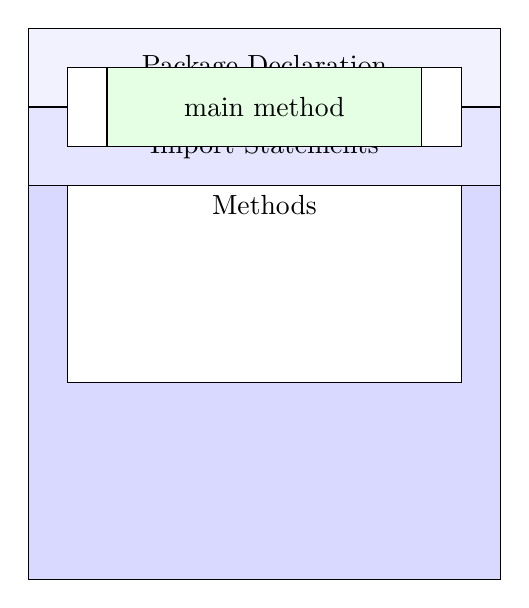
\begin{tikzpicture}[node distance=0cm, outer sep=0pt]
    \node [draw, rectangle, minimum width=6cm, minimum height=1cm, fill=blue!5] (pkg) {Package Declaration};
    \node [draw, rectangle, minimum width=6cm, minimum height=1cm, below=0cm of pkg, fill=blue!10] (imp) {Import Statements};
    
    \node [draw, rectangle, minimum width=6cm, minimum height=5cm, below=0cm of imp, fill=blue!15, label={[anchor=north]north:Class Declaration}] (cls) {};
    
    \node [draw, rectangle, minimum width=5cm, minimum height=1cm, below=-1.5cm of cls.north, fill=white] (var) {Variables};
    \node [draw, rectangle, minimum width=5cm, minimum height=2.5cm, below=0.5cm of var, fill=white, label={[anchor=north]north:Methods}] (mtd) {};
    
    \node [draw, rectangle, minimum width=4cm, minimum height=1cm, below=-1.5cm of mtd.north, fill=green!10] (main) {main method};

\end{tikzpicture}
\captionof{figure}{Structure of Java Program}
\end{center}

\begin{itemize}
    \item \textbf{Package}: Groups related classes (e.g., \code{package com.example;})
    \item \textbf{Import}: Access libraries (e.g., \code{import java.util.*;})
    \item \textbf{Class}: Contains all code
    \item \textbf{Main method}: Execution starts here
\end{itemize}
\end{solutionbox}

\begin{mnemonicbox}
\mnemonic{PICM - Package, Import, Class, Main}
\end{mnemonicbox}

\questionmarks{1(b)}{4}{List out different features of java. Explain any two.}

\begin{solutionbox}
\textbf{Java Features}:
\begin{enumerate}
    \item \textbf{Platform Independent}: Write Once, Run Anywhere (WORA)
    \item \textbf{Object Oriented}: Everything is an object
    \item \textbf{Simple}: No complex features like pointers
    \item \textbf{Secure}: Bytecode verification, no explicit memory access
    \item \textbf{Robust}: Strong memory management, exception handling
    \item \textbf{Multithreaded}: Concurrent execution support
\end{enumerate}

\textbf{1. Platform Independence:}
Java programs are compiled into bytecode, which is platform-neutral. This bytecode is interpreted by the Java Virtual Machine (JVM) specific to each operating system (Windows, Linux, Mac), allowing the same code to run everywhere without recompilation.

\textbf{2. Object Oriented:}
Java models real-world entities using objects and classes. It supports key OOP principles:
\begin{itemize}
    \item \textbf{Encapsulation}: bundling data and methods
    \item \textbf{Inheritance}: code reusability
    \item \textbf{Polymorphism}: same interface, multiple forms
\end{itemize}
\end{solutionbox}

\begin{mnemonicbox}
\mnemonic{POSRMM - Platform, Object, Simple, Robust, Multithreaded, Memory}
\end{mnemonicbox}

\questionmarks{1(c)}{7}{Write a program in java to find out sum of the digits of entered number. (Ex. Number is 123 output is 6).}

\begin{solutionbox}
\begin{lstlisting}[language=Java,caption={Sum of Digits}]
public class DigitSum {
    public static void main(String[] args) {
        if (args.length == 0) {
            System.out.println("Please provide a number.");
            return;
        }
        
        int number = Integer.parseInt(args[0]);
        int sum = 0;
        int temp = Math.abs(number);
        
        // Loop to extract and add digits
        while (temp > 0) {
            sum += temp % 10;  // Extract last digit
            temp /= 10;        // Remove last digit
        }
        
        System.out.println("Sum of digits: " + sum);
    }
}
\end{lstlisting}

\begin{center}
\captionof{table}{Algorithm Trace (Input: 123)}
\begin{tabulary}{\linewidth}{|L|L|L|}
\hline
\textbf{Step} & \textbf{Operation} & \textbf{Result} \\ \hline
1 & Extract digit & $123 \% 10 = 3$ \\ \hline
2 & Add to sum & $sum = 0 + 3 = 3$ \\ \hline
3 & Remove digit & $123 / 10 = 12$ \\ \hline
4 & Extract digit & $12 \% 10 = 2$ \\ \hline
5 & Add to sum & $sum = 3 + 2 = 5$ \\ \hline
6 & Remove digit & $12 / 10 = 1$ \\ \hline
7 & Extract digit & $1 \% 10 = 1$ \\ \hline
8 & Add to sum & $sum = 5 + 1 = 6$ \\ \hline
\end{tabulary}
\end{center}
\end{solutionbox}

\begin{mnemonicbox}
\mnemonic{EARD - Extract, Add, Remove, Done}
\end{mnemonicbox}

\questionmarks{1(c OR)}{7}{Write a program in java to find out maximum from any ten numbers using command line argument.}

\begin{solutionbox}
\begin{lstlisting}[language=Java,caption={Find Maximum from Arguments}]
public class FindMaximum {
    public static void main(String[] args) {
        if (args.length < 10) {
            System.out.println("Please enter 10 numbers");
            return;
        }
        
        // Initialize max with the first number
        int max = Integer.parseInt(args[0]);
        
        // Loop through remaining numbers
        for (int i = 1; i < 10; i++) {
            int current = Integer.parseInt(args[i]);
            if (current > max) {
                max = current;
            }
        }
        
        System.out.println("Maximum number: " + max);
    }
}
\end{lstlisting}

\begin{center}
\captionof{table}{Logic Steps}
\begin{tabulary}{\linewidth}{|L|L|}
\hline
\textbf{Step} & \textbf{Action} \\ \hline
Validation & Check if at least 10 arguments are provided \\ \hline
Initialization & Assume first argument is \code{max} \\ \hline
Comparison & Loop through remaining 9 numbers \\ \hline
Update & If \code{current > max}, set \code{max = current} \\ \hline
Output & Print the final \code{max} value \\ \hline
\end{tabulary}
\end{center}
\end{solutionbox}

\begin{mnemonicbox}
\mnemonic{VCIU - Validate, Compare, Initialize, Update}
\end{mnemonicbox}

\questionmarks{2(a)}{3}{List out different concept of oop. Explain anyone in detail.}

\begin{solutionbox}
\textbf{OOP Concepts}:
\begin{itemize}
    \item Encapsulation
    \item Inheritance
    \item Polymorphism
    \item Abstraction
\end{itemize}

\textbf{Encapsulation}:
Encapsulation is the mechanism of wrapping code (methods) and data (variables) together into a single unit (class). It protects data from outside interference and misuse.

\begin{itemize}
    \item \textbf{Data Hiding}: Variables are declared \code{private} to restrict direct access.
    \item \textbf{Accessors/Mutators}: Public \code{getter} and \code{setter} methods are provided to access and modify data controllably.
    \item \textbf{Benefits}: Improves security, modularity, and maintainability.
\end{itemize}
\end{solutionbox}

\begin{mnemonicbox}
\mnemonic{EIPA - Encapsulation, Inheritance, Polymorphism, Abstraction}
\end{mnemonicbox}

\questionmarks{2(b)}{4}{Explain JVM in detail.}

\begin{solutionbox}
\textbf{JVM (Java Virtual Machine)} is the engine that executes Java bytecode. It provides a runtime environment for Java code.

\begin{center}
\begin{tikzpicture}[auto, node distance=1.5cm]
    \node [gtu block] (source) {Java Source};
    \node [gtu block, right=of source] (compiler) {Compiler};
    \node [gtu block, right=of compiler] (bytecode) {Bytecode};
    \node [gtu block, below=1cm of compiler, fill=yellow!10, minimum width=4cm] (jvm) {JVM};
    
    \node [gtu block, below=0.5cm of jvm] (os) {Native OS};
    
    \draw [gtu arrow] (source) -- (compiler);
    \draw [gtu arrow] (compiler) -- (bytecode);
    \draw [gtu arrow] (bytecode) -- (jvm);
    \draw [gtu arrow] (jvm) -- (os);
    
    % Internal JVM components
    \node [draw, dashed, inner sep=5pt, fit=(jvm)] {}; 
    \node [right=0.2cm of jvm, text width=3cm, font=\footnotesize] {
    Includes:\\
    - Class Loader\\
    - Memory Areas\\
    - Execution Engine};
\end{tikzpicture}
\captionof{figure}{JVM Architecture}
\end{center}

\begin{center}
\captionof{table}{JVM Components}
\begin{tabulary}{\linewidth}{|L|L|}
\hline
\textbf{Component} & \textbf{Function} \\ \hline
Class Loader & Loads \code{.class} files into memory \\ \hline
Memory Areas & Allocates memory (Heap, Stack, Method Area) \\ \hline
Execution Engine & Interprets bytecode or uses JIT compiler \\ \hline
JIT Compiler & Compiles hot code to native machine code for speed \\ \hline
\end{tabulary}
\end{center}

\textbf{Key Features}:
\begin{itemize}
    \item \textbf{Platform Independence}: JVM makes Java portable.
    \item \textbf{Memory Management}: Handles allocation and garbage collection.
\end{itemize}
\end{solutionbox}

\begin{mnemonicbox}
\mnemonic{CEMJ - Class loader, Execution, Memory, JIT}
\end{mnemonicbox}

\questionmarks{2(c)}{7}{Explain constructor overloading with example.}

\begin{solutionbox}
\textbf{Constructor Overloading}: A technique of having more than one constructor in a class with different parameter lists.

\begin{lstlisting}[language=Java,caption={Constructor Overloading}]
public class Student {
    private String name;
    private int age;
    private String course;
    
    // 1. Default constructor
    public Student() {
        this.name = "Unknown";
        this.age = 0;
        this.course = "Not Assigned";
    }
    
    // 2. Constructor with one parameter
    public Student(String name) {
        this.name = name;
        this.age = 0;
        this.course = "Not Assigned";
    }
    
    // 3. Constructor with two parameters
    public Student(String name, int age) {
        this.name = name;
        this.age = age;
        this.course = "Not Assigned";
    }
    
    // 4. Constructor with all parameters
    public Student(String name, int age, String course) {
        this.name = name;
        this.age = age;
        this.course = course;
    }
}
\end{lstlisting}

\begin{center}
\captionof{table}{Types of Constructors in Example}
\begin{tabulary}{\linewidth}{|L|L|L|}
\hline
\textbf{Constructor} & \textbf{Parameters} & \textbf{Purpose} \\ \hline
Default & None & Initialize with default values \\ \hline
Single Param & Name & Register student with just name \\ \hline
Two Param & Name, Age & Register with basic details \\ \hline
Full Param & All fields & Complete initialization \\ \hline
\end{tabulary}
\end{center}

\textbf{Rules}:
\begin{itemize}
    \item Must have the same name as the class.
    \item Must have different parameter lists (number or type of args).
    \item Resolved at compile-time (Compile-time Polymorphism).
\end{itemize}
\end{solutionbox}

\begin{mnemonicbox}
\mnemonic{SNDF - Same Name, Different Parameters, Flexible}
\end{mnemonicbox}

\questionmarks{2(a OR)}{3}{What is wrapper class? Explain with example.}

\begin{solutionbox}
\textbf{Wrapper Class}: A class whose object wraps or contains a primitive data type. They convert primitive data types into objects.

\begin{center}
\captionof{table}{Primitive vs Wrapper}
\begin{tabulary}{\linewidth}{|L|L|}
\hline
\textbf{Primitive} & \textbf{Wrapper Class} \\ \hline
byte & Byte \\ \hline
int & Integer \\ \hline
char & Character \\ \hline
double & Double \\ \hline
boolean & Boolean \\ \hline
\end{tabulary}
\end{center}

\begin{lstlisting}[language=Java,caption={Boxing and Unboxing}]
// Boxing: Primitive to Object
int num = 10;
Integer obj = Integer.valueOf(num); // Manual
Integer autoBox = 10;               // Autoboxing

// Unboxing: Object to Primitive
Integer wrapper = new Integer(20);
int value = wrapper.intValue();     // Manual
int autoUnbox = wrapper;            // Auto-unboxing
\end{lstlisting}

\textbf{Usage}: Required in Collection Frameworks (ArrayList, Vector) where only objects are stored.
\end{solutionbox}

\begin{mnemonicbox}
\mnemonic{BUC - Boxing, Unboxing, Collections}
\end{mnemonicbox}

\questionmarks{2(b OR)}{4}{Explain static keyword with example.}

\begin{solutionbox}
\textbf{Static Keyword}: Indicates that a member belongs to the class type itself, rather than to an instance of that class.

\begin{center}
\captionof{table}{Static Uses}
\begin{tabulary}{\linewidth}{|L|L|}
\hline
\textbf{Member} & \textbf{Behavior} \\ \hline
Variable & Shared memory among all instances (class variable) \\ \hline
Method & Can be called without creating an object \\ \hline
Block & Executed once when class is loaded \\ \hline
\end{tabulary}
\end{center}

\begin{lstlisting}[language=Java,caption={Static Example}]
public class Counter {
    static int count = 0;  // Shared variable
    int id;                // Instance variable
    
    public Counter() {
        count++;           // Increments for every new object
        this.id = count;
    }
    
    public static void showCount() {
        // Can only access static data
        System.out.println("Total objects: " + count);
    }
}
\end{lstlisting}

\begin{itemize}
    \item \textbf{Memory Efficiency}: Variable created only once.
    \item \textbf{Utility}: Used for utility methods (e.g., \code{Math.sqrt()}).
\end{itemize}
\end{solutionbox}

\begin{mnemonicbox}
\mnemonic{SCMA - Shared, Class-level, Memory, Access}
\end{mnemonicbox}

\questionmarks{2(c OR)}{7}{What is constructor? Explain copy constructor with example.}

\begin{solutionbox}
\textbf{Constructor}: A special block of code used to initialize an object. It is called when an instance of the class is created.

\textbf{Copy Constructor}: A constructor that initializes an object using another object of the same class. It creates a clone of the existing object.

\begin{lstlisting}[language=Java,caption={Copy Constructor}]
public class Book {
    private String title;
    private String author;
    
    // Parameterized constructor
    public Book(String title, String author) {
        this.title = title;
        this.author = author;
    }
    
    // Copy constructor
    public Book(Book other) {
        this.title = other.title;
        this.author = other.author;
    }
    
    public void display() {
        System.out.println(title + " by " + author);
    }
}

// Usage
class Main {
    public static void main(String[] args) {
        Book b1 = new Book("Java Guide", "James");
        Book b2 = new Book(b1); // Creates a copy of b1
        b1.display();
        b2.display();
    }
}
\end{lstlisting}

\begin{center}
\captionof{table}{Constructor Properties}
\begin{tabulary}{\linewidth}{|L|L|}
\hline
\textbf{Property} & \textbf{Description} \\ \hline
Name & Must match class name \\ \hline
Return Type & None (not even void) \\ \hline
Invocation & Automatic at time of \code{new} \\ \hline
\end{tabulary}
\end{center}
\end{solutionbox}

\begin{mnemonicbox}
\mnemonic{SNAC - Same Name, Automatic Call}
\end{mnemonicbox}

\questionmarks{3(a)}{3}{Explain any four-string function in java with example.}

\begin{solutionbox}
\textbf{String Functions}:
\begin{center}
\captionof{table}{Common String Functions}
\begin{tabulary}{\linewidth}{|L|L|L|}
\hline
\textbf{Function} & \textbf{Purpose} & \textbf{Example} \\ \hline
\code{length()} & Returns number of characters & \code{"Hi".length()} $\to$ 2 \\ \hline
\code{charAt(i)} & Returns char at index i & \code{"Hi".charAt(0)} $\to$ 'H' \\ \hline
\code{substring(i)} & Returns part of string from i & \code{"Code".substring(2)} $\to$ "de" \\ \hline
\code{toUpperCase()} & Converts to uppercase & \code{"java".toUpperCase()} $\to$ "JAVA" \\ \hline
\end{tabulary}
\end{center}

\begin{lstlisting}[language=Java,caption={String Example}]
String str = "Java Programming";
int len = str.length();           // 16
char ch = str.charAt(0);          // 'J'
String sub = str.substring(5);    // "Programming"
String upper = str.toUpperCase(); // "JAVA PROGRAMMING"
\end{lstlisting}
\end{solutionbox}

\begin{mnemonicbox}
\mnemonic{LCST - Length, Character, Substring, Transform}
\end{mnemonicbox}

\questionmarks{3(b)}{4}{List out different types of inheritance. Explain multilevel inheritance.}

\begin{solutionbox}
\textbf{Types of Inheritance}:
\begin{enumerate}
    \item Single Inheritance
    \item Multilevel Inheritance
    \item Hierarchical Inheritance
    \item Multiple Inheritance (via Interfaces)
    \item Hybrid Inheritance
\end{enumerate}

\textbf{Multilevel Inheritance}:
A mechanism where a class inherits from a derived class, forming a chain of inheritance.

\begin{center}
\begin{tikzpicture}[node distance=1.5cm]
    \node [gtu block] (veh) {Vehicle};
    \node [gtu block, right=of veh] (car) {Car};
    \node [gtu block, right=of car] (sports) {SportsCar};
    
    \draw [gtu arrow] (veh) -- (car);
    \draw [gtu arrow] (car) -- (sports);
\end{tikzpicture}
\captionof{figure}{Multilevel Inheritance}
\end{center}

\begin{lstlisting}[language=Java,caption={Multilevel Inheritance}]
class Vehicle { void start() {} }
class Car extends Vehicle { void drive() {} }
class SportsCar extends Car { void race() {} }
\end{lstlisting}

In this example, \code{SportsCar} inherits features from both \code{Car} and \code{Vehicle}.
\end{solutionbox}

\begin{mnemonicbox}
\mnemonic{SMHM - Single, Multilevel, Hierarchical, Multiple}
\end{mnemonicbox}

\questionmarks{3(c)}{7}{What is interface? Explain multiple inheritance with example.}

\begin{solutionbox}
\textbf{Interface}: An abstract reference type in Java that is similar to a class but contains only constants, method signatures (empty methods), default methods, and static methods. It is used to achieve total abstraction and multiple inheritance.

\textbf{Multiple Inheritance}: Java does not support multiple inheritance with classes to avoid ambiguity (Diamond Problem), but it supports it through interfaces. A class can implement multiple interfaces.

\begin{center}
\begin{tikzpicture}[node distance=2cm]
    \node [gtu block] (fly) {interface Flyable};
    \node [gtu block, right=of fly] (swim) {interface Swimmable};
    \node [gtu block, below right=1cm and -1cm of fly] (duck) {class Duck};
    
    \draw [gtu arrow] (fly) -- (duck);
    \draw [gtu arrow] (swim) -- (duck);
\end{tikzpicture}
\captionof{figure}{Multiple Inheritance via Interfaces}
\end{center}

\begin{lstlisting}[language=Java,caption={Multiple Inheritance Example}]
interface Flyable {
    void fly();
}
interface Swimmable {
    void swim();
}

// Single class implementing multiple interfaces
class Duck implements Flyable, Swimmable {
    public void fly() {
        System.out.println("Duck is flying");
    }
    public void swim() {
        System.out.println("Duck is swimming");
    }
}
\end{lstlisting}

\begin{center}
\captionof{table}{Interface vs Class}
\begin{tabulary}{\linewidth}{|L|L|}
\hline
\textbf{Interface} & \textbf{Class} \\ \hline
Can contain abstract methods & Contains concrete methods \\ \hline
Variables are \code{public static final} & Any variable type allowed \\ \hline
Supports multiple inheritance & Supports single inheritance \\ \hline
\end{tabulary}
\end{center}
\end{solutionbox}

\begin{mnemonicbox}
\mnemonic{CMDS - Contract, Multiple, Diamond-solution}
\end{mnemonicbox}

\questionmarks{3(a OR)}{3}{Explain this keyword with example.}

\begin{solutionbox}
\textbf{'this' Keyword}: A reference variable in Java that refers to the current object.

\begin{center}
\captionof{table}{Uses of 'this'}
\begin{tabulary}{\linewidth}{|L|L|}
\hline
\textbf{Use Case} & \textbf{Purpose} \\ \hline
Instance Variable & Distinguish field from parameter (\code{this.x = x}) \\ \hline
Method Call & Invoke current class method (\code{this.method()}) \\ \hline
Constructor Call & Chain constructors (\code{this()}) \\ \hline
Return Object & Return current instance (\code{return this}) \\ \hline
\end{tabulary}
\end{center}

\begin{lstlisting}[language=Java,caption={Using 'this'}]
public class Person {
    String name;
    
    public Person(String name) {
        this.name = name; // Resolves ambiguity
    }
    
    public Person getInstance() {
        return this; // Returns current object
    }
}
\end{lstlisting}
\end{solutionbox}

\begin{mnemonicbox}
\mnemonic{CRPM - Current, Resolve, Parameter, Method}
\end{mnemonicbox}

\questionmarks{3(b OR)}{4}{Explain method overriding with example.}

\begin{solutionbox}
\textbf{Method Overriding}: Occurs when a subclass provides a specific implementation for a method that is already defined in its parent class. It is used for Runtime Polymorphism.

\begin{lstlisting}[language=Java,caption={Method Overriding}]
class Animal {
    void makeSound() {
        System.out.println("Animal makes sound");
    }
}

class Dog extends Animal {
    @Override
    void makeSound() {
        System.out.println("Dog barks");
    }
}

class Main {
    public static void main(String[] args) {
        Animal a = new Dog(); // Upcasting
        a.makeSound(); // Output: Dog barks
    }
}
\end{lstlisting}

\begin{center}
\captionof{table}{Overriding Rules}
\begin{tabulary}{\linewidth}{|L|L|}
\hline
\textbf{Rule} & \textbf{Description} \\ \hline
Signature & Method name and args must be identical \\ \hline
Inheritance & Must involve IS-A relationship \\ \hline
Access & Access level cannot be more restrictive \\ \hline
Binding & Resolved at runtime (Dynamic Binding) \\ \hline
\end{tabulary}
\end{center}
\end{solutionbox}

\begin{mnemonicbox}
\mnemonic{SSRD - Same Signature, Runtime Decision}
\end{mnemonicbox}

\questionmarks{3(c OR)}{7}{What is package? Write steps to create a package and give example of it.}

\begin{solutionbox}
\textbf{Package}: A namespace that organizes a set of related classes and interfaces. It helps in:
\begin{itemize}
    \item Preventing naming conflicts.
    \item Controlling access (protected/default access).
    \item Making searching/usage of classes easier.
\end{itemize}

\textbf{Steps to Create and Use a Package}:
\begin{enumerate}
    \item \textbf{Directory}: Create a folder structure matching the package name (e.g., \code{com/utils}).
    \item \textbf{Declaration}: Add \code{package com.utils;} at the top of the file.
    \item \textbf{Compile}: Compile with \code{-d .} to generate folders automatically.
    \item \textbf{Import}: Use \code{import com.utils.*;} in another file.
\end{enumerate}

\begin{lstlisting}[language=Java,caption={Creating a Package}]
// File: src/com/company/utils/MathUtils.java
package com.company.utils;

public class MathUtils {
    public static int add(int a, int b) {
        return a + b;
    }
}
\end{lstlisting}

\begin{lstlisting}[language=Java,caption={Using a Package}]
// File: src/Calculator.java
import com.company.utils.MathUtils;

public class Calculator {
    public static void main(String[] args) {
        int result = MathUtils.add(5, 10);
        System.out.println("Result: " + result);
    }
}
\end{lstlisting}

\begin{center}
\captionof{table}{Compiling and Running}
\begin{tabulary}{\linewidth}{|L|L|}
\hline
\textbf{Action} & \textbf{Command} \\ \hline
Compile Package & \code{javac -d . MathUtils.java} \\ \hline
Compile Main & \code{javac Calculator.java} \\ \hline
Run & \code{java Calculator} \\ \hline
\end{tabulary}
\end{center}
\end{solutionbox}

\begin{mnemonicbox}
\mnemonic{ONAM - Organization, Namespace, Access, Maintenance}
\end{mnemonicbox}

\questionmarks{4(a)}{3}{Explain thread priorities with suitable example.}

\begin{solutionbox}
\textbf{Thread Priority}: Java threads have priority values from 1 to 10 that help the Thread Scheduler decide which thread to execute.

\begin{center}
\captionof{table}{Priority Constants}
\begin{tabulary}{\linewidth}{|L|L|L|}
\hline
\textbf{Level} & \textbf{Constant} & \textbf{Value} \\ \hline
Min & \code{Thread.MIN\_PRIORITY} & 1 \\ \hline
Norm & \code{Thread.NORM\_PRIORITY} & 5 (Default) \\ \hline
Max & \code{Thread.MAX\_PRIORITY} & 10 \\ \hline
\end{tabulary}
\end{center}

\begin{lstlisting}[language=Java,caption={Thread Priority}]
class MyThread extends Thread {
    public void run() {
        System.out.println("Running: " + getName());
    }
}

public class PriorityDemo {
    public static void main(String[] args) {
        MyThread t1 = new MyThread();
        MyThread t2 = new MyThread();
        
        t1.setPriority(Thread.MAX_PRIORITY); // 10
        t2.setPriority(Thread.MIN_PRIORITY); // 1
        
        t1.start(); // Likely to run first
        t2.start();
    }
}
\end{lstlisting}
\end{solutionbox}

\begin{mnemonicbox}
\mnemonic{HNG - Higher priority, Not Guaranteed}
\end{mnemonicbox}

\questionmarks{4(b)}{4}{What is Thread? Explain Thread life cycle.}

\begin{solutionbox}
\textbf{Thread}: A lightweight subprocess that runs concurrently with other threads.

\textbf{Thread Life Cycle}: A thread goes through various states during its lifetime.

\begin{center}
\begin{tikzpicture}[node distance=2cm, auto, >=stealth]
    \node [gtu state] (new) {NEW};
    \node [gtu state, right=of new] (runnable) {RUNNABLE};
    \node [gtu state, right=of runnable] (running) {RUNNING};
    \node [gtu state, right=of running] (term) {TERMINATED};
    \node [gtu state, below=of running] (blocked) {BLOCKED/WAITING};
    
    \draw [->, thick] (new) -- node[above] {\small start()} (runnable);
    \draw [->, thick] (runnable) -- node[above] {\small Scheduler} (running);
    \draw [->, thick] (running) -- node[above] {\small End} (term);
    \draw [->, thick] (running) -- node[right] {\small sleep/wait} (blocked);
    \draw [->, thick] (blocked) -| node[below, near start] {\small notify/time} (runnable);
\end{tikzpicture}
\captionof{figure}{Thread Life Cycle}
\end{center}

\begin{center}
\captionof{table}{Thread States}
\begin{tabulary}{\linewidth}{|L|L|}
\hline
\textbf{State} & \textbf{Description} \\ \hline
NEW & Created instance, \code{start()} not called \\ \hline
RUNNABLE & Ready to run, waiting for CPU \\ \hline
RUNNING & Currently executing \\ \hline
BLOCKED & Waiting for resource explicitly \\ \hline
TERMINATED & Executed finished \\ \hline
\end{tabulary}
\end{center}
\end{solutionbox}

\begin{mnemonicbox}
\mnemonic{NRBT - New, Runnable, Blocked, Terminated}
\end{mnemonicbox}

\questionmarks{4(c)}{7}{Write a program in java that create the multiple threads by implementing the Thread class.}

\begin{solutionbox}
\begin{lstlisting}[language=Java,caption={Multiple Threads}]
class NumberPrinter extends Thread {
    String name;
    
    NumberPrinter(String name) {
        this.name = name;
    }
    
    public void run() {
        for(int i=1; i<=3; i++) {
            System.out.println(name + ": " + i);
            try { 
                Thread.sleep(500); // Pause
            } catch(Exception e) {}
        }
    }
}

public class MultiThreadDemo {
    public static void main(String[] args) {
        NumberPrinter t1 = new NumberPrinter("Thread-1");
        NumberPrinter t2 = new NumberPrinter("Thread-2");
        NumberPrinter t3 = new NumberPrinter("Thread-3");
        
        // Start all threads concurrently
        t1.start();
        t2.start();
        t3.start();
        
        System.out.println("Main finished");
    }
}
\end{lstlisting}

\textbf{Steps}:
\begin{enumerate}
    \item Extend \code{Thread} class.
    \item Override \code{run()} method with logic.
    \item Create instances of the class.
    \item Call \code{start()} to begin execution.
\end{enumerate}
\end{solutionbox}

\begin{mnemonicbox}
\mnemonic{EOCS - Extend, Override, Create, Start}
\end{mnemonicbox}

\questionmarks{4(a OR)}{3}{Explain basic concept of Exception Handling.}

\begin{solutionbox}
\textbf{Exception Handling}: A mechanism to handle runtime errors so that the normal flow of the application can be maintained.

\begin{center}
\captionof{table}{Key Blocks}
\begin{tabulary}{\linewidth}{|L|L|}
\hline
\textbf{Keyword} & \textbf{Function} \\ \hline
try & Block of code to monitor for errors \\ \hline
catch & Block that handles the exception \\ \hline
finally & Block that executes regardless of outcome \\ \hline
throw & Used to explicitly throw an exception \\ \hline
throws & Declares exceptions a method can throw \\ \hline
\end{tabulary}
\end{center}

\begin{lstlisting}[language=Java,caption={Exception Syntax}]
try {
    // Risky code
} catch (Exception e) {
    // Handling code
} finally {
    // Cleanup
}
\end{lstlisting}
\end{solutionbox}

\begin{mnemonicbox}
\mnemonic{TRCF - Try, Runtime error, Catch, Finally}
\end{mnemonicbox}

\questionmarks{4(b OR)}{4}{Explain multiple catch with suitable example.}

\begin{solutionbox}
\textbf{Multiple Catch Blocks}: A \code{try} block can be followed by multiple \code{catch} blocks to handle different types of exceptions separately.

\begin{lstlisting}[language=Java,caption={Multiple Catch}]
public class MultiCatch {
    public static void main(String[] args) {
        try {
            int a[] = new int[5];
            a[10] = 30 / 0; // Risky code
        } catch (ArithmeticException e) {
            System.out.println("Math Error: " + e);
        } catch (ArrayIndexOutOfBoundsException e) {
            System.out.println("Array Error: " + e);
        } catch (Exception e) {
            // Generic catch must be last
            System.out.println("General Error: " + e);
        }
    }
}
\end{lstlisting}

\textbf{Rules}:
\begin{itemize}
    \item At a time only one exception occurs and only one catch block is executed.
    \item Specific exceptions must be caught before general exceptions (\code{Exception} parent class).
\end{itemize}
\end{solutionbox}

\begin{mnemonicbox}
\mnemonic{SOOF - Specific first, One executes, Order matters, Finally}
\end{mnemonicbox}

\questionmarks{4(c OR)}{7}{What is Exception? Write a program that show the use of Arithmetic Exception.}

\begin{solutionbox}
\textbf{Exception}: An unwanted or unexpected event that occurs during the execution of a program (at runtime) that disrupts the normal flow of instructions.

\textbf{ArithmeticException}: A runtime exception thrown when an exceptional arithmetic condition has occurred, such as division by zero.

\begin{lstlisting}[language=Java,caption={Arithmetic Exception Demo}]
public class DivisionDemo {
    public static void main(String[] args) {
        System.out.println("Start of program");
        
        try {
            int numerator = 100;
            int denominator = 0; // Division by zero
            
            // This line throws ArithmeticException
            int result = numerator / denominator;
            
            System.out.println("Result: " + result);
        } catch (ArithmeticException e) {
            System.out.println("Error detected: Division by zero is not allowed.");
            System.out.println("Exception: " + e.getMessage());
        } finally {
            System.out.println("Cleanup actions...");
        }
        
        System.out.println("Program continues normally...");
    }
}
\end{lstlisting}

\textbf{Output}:
\begin{verbatim}
Start of program
Error detected: Division by zero is not allowed.
Exception: / by zero
Cleanup actions...
Program continues normally...
\end{verbatim}

Without the try-catch block, the program would crash immediately at the point of division.
\end{solutionbox}

\begin{mnemonicbox}
\mnemonic{DZMI - Division by Zero, Mathematical Invalid}
\end{mnemonicbox}

\questionmarks{5(a)}{3}{Explain ArrayIndexOutOfBound Exception in Java with example.}

\begin{solutionbox}
\textbf{ArrayIndexOutOfBoundsException}: A runtime exception thrown to indicate that an array has been accessed with an illegal index. The index is either negative or greater than or equal to the size of the array.

\begin{center}
\captionof{table}{Causes}
\begin{tabulary}{\linewidth}{|L|L|L|}
\hline
\textbf{Cause} & \textbf{Description} & \textbf{Example} \\ \hline
Negative Index & Index $< 0$ & a[-1] \\ \hline
Size Exceeded & Index $\ge$ Length & a[length] \\ \hline
Empty Array & Accessing index 0 of empty & a[0] \\ \hline
\end{tabulary}
\end{center}

\begin{lstlisting}[language=Java,caption={Array Index Exception}]
int[] numbers = {10, 20, 30}; // Size 3, indices 0-2
try {
    System.out.println(numbers[5]); // Index 5 is invalid
} catch (ArrayIndexOutOfBoundsException e) {
    System.out.println("Invalid Index: " + e.getMessage());
}
\end{lstlisting}
\end{solutionbox}

\begin{mnemonicbox}
\mnemonic{NIE - Negative, Index-exceed, Empty}
\end{mnemonicbox}

\questionmarks{5(b)}{4}{Explain basics of stream classes.}

\begin{solutionbox}
\textbf{Stream Classes}: A stream is a sequence of data. Java I/O is based on streams.

\begin{center}
\begin{tikzpicture}[node distance=1cm, level 1/.style={sibling distance=5cm}, level 2/.style={sibling distance=2.5cm}]
    \node [gtu block] {Java I/O}
        child {node [gtu block] {Byte Stream}
            child {node [gtu block] {InputStream}}
            child {node [gtu block] {OutputStream}}
        }
        child {node [gtu block] {Character Stream}
            child {node [gtu block] {Reader}}
            child {node [gtu block] {Writer}}
        };
\end{tikzpicture}
\captionof{figure}{Stream Hierarchy}
\end{center}

\begin{center}
\captionof{table}{Stream Categories}
\begin{tabulary}{\linewidth}{|L|L|L|}
\hline
\textbf{Stream Type} & \textbf{Data Type} & \textbf{Classes} \\ \hline
Byte Stream & Binary Data (Images, etc) & InputStream, OutputStream \\ \hline
Char Stream & Text Data (Strings) & Reader, Writer \\ \hline
\end{tabulary}
\end{center}

\textbf{Subclasses}:
\begin{itemize}
    \item \textbf{File}: FileInputStream, FileWriter, etc.
    \item \textbf{Buffered}: BufferedReader, BufferedOutputStream (for efficiency).
\end{itemize}
\end{solutionbox}

\begin{mnemonicbox}
\mnemonic{BCIF - Byte, Character, Input/Output, File}
\end{mnemonicbox}

\questionmarks{5(c)}{7}{Write a java program to create a text file and perform write operation on the text file.}

\begin{solutionbox}
\begin{lstlisting}[language=Java,caption={Write to File}]
import java.io.FileWriter;
import java.io.IOException;

public class FileWriteDemo {
    public static void main(String[] args) {
        // Data to write
        String data = "This is a sample text file created by Java program.\nWelcome to Summer 2024 Solution.";
        
        // Using Try-with-resources to automatically close the writer
        try (FileWriter writer = new FileWriter("output.txt")) {
            
            // Writing data
            writer.write(data);
            
            System.out.println("Successfully wrote to the file.");
            
        } catch (IOException e) {
            System.out.println("An error occurred.");
            e.printStackTrace();
        }
    }
}
\end{lstlisting}

\textbf{Explanation}:
\begin{enumerate}
    \item \textbf{Import}: \code{java.io.FileWriter} and \code{IOException}.
    \item \textbf{FileWriter}: Creates a file writer object. Pass file name string.
    \item \textbf{write()}: Method to write string content to the file.
    \item \textbf{close()}: Automatically called by try-with-resources block to save data and free resources.
\end{enumerate}

\begin{center}
\captionof{table}{Methods Used}
\begin{tabulary}{\linewidth}{|L|L|}
\hline
\textbf{Method} & \textbf{Description} \\ \hline
FileWriter(String) & Creates new file, overwrites if exists \\ \hline
write(String) & Writes text to stream \\ \hline
close() & Flushes and closes stream \\ \hline
\end{tabulary}
\end{center}
\end{solutionbox}

\begin{mnemonicbox}
\mnemonic{CWCH - Create, Write, Close, Handle}
\end{mnemonicbox}

\questionmarks{5(a OR)}{3}{Explain Divide by Zero Exception in Java with example.}

\begin{solutionbox}
\textbf{Divide by Zero}: Trying to divide an integer by zero is an illegal operation in Java.

\begin{center}
\captionof{table}{Behavior}
\begin{tabulary}{\linewidth}{|L|L|L|}
\hline
\textbf{Case} & \textbf{Result} & \textbf{Exception} \\ \hline
Integer / 0 & Illegal & ArithmeticException \\ \hline
Float / 0.0 & Infinity & None \\ \hline
Modulo \% 0 & Illegal & ArithmeticException \\ \hline
\end{tabulary}
\end{center}

\begin{lstlisting}[language=Java,caption={Divide By Zero}]
try {
    int a = 10 / 0; // Throws Exception
} catch (ArithmeticException e) {
    System.out.println("Cannot divide integer by zero");
}

double b = 10.0 / 0.0;
System.out.println(b); // Prints "Infinity"
\end{lstlisting}
\end{solutionbox}

\begin{mnemonicbox}
\mnemonic{IFM - Integer exception, Float infinity, Modulo error}
\end{mnemonicbox}

\questionmarks{5(b OR)}{4}{Explain try and catch block with example.}

\begin{solutionbox}
\textbf{Try-Catch}: The core mechanism for exception handling.

\begin{itemize}
    \item \textbf{try}: Encloses the code that might generate an exception.
    \item \textbf{catch}: Defines how to handle the exception. It must follow a try block.
\end{itemize}

\begin{lstlisting}[language=Java,caption={Try-Catch Example}]
public class Example {
    public static void main(String args[]) {
        try {
            String s = null;
            System.out.println(s.length()); // NullPointer
        } catch(NullPointerException e) {
            System.out.println("Caught Null Pointer Exception");
        }
        
        System.out.println("Rest of the code...");
    }
}
\end{lstlisting}

\begin{center}
\captionof{table}{Program Flow}
\begin{tabulary}{\linewidth}{|L|L|}
\hline
\textbf{Scenario} & \textbf{Execution Path} \\ \hline
No Exception & try executes -> catch skipped -> rest of code \\ \hline
Exception & try stops at error -> catch executes -> rest of code \\ \hline
\end{tabulary}
\end{center}
\end{solutionbox}

\begin{mnemonicbox}
\mnemonic{TCF - Try risky, Catch exception, Finally cleanup}
\end{mnemonicbox}

\questionmarks{5(c OR)}{7}{Write a java program to display the content of a text file and perform append operation on the text file.}

\begin{solutionbox}
\begin{lstlisting}[language=Java,caption={Read and Append}]
import java.io.*;

public class FileReadAppend {
    public static void main(String[] args) {
        String filename = "log.txt";
        
        // 1. Append Operation
        try (FileWriter fw = new FileWriter(filename, true);
             BufferedWriter bw = new BufferedWriter(fw)) {
            
            bw.write("New Log Entry\n");
            System.out.println("Appended to file.");
            
        } catch (IOException e) {
            e.printStackTrace();
        }
        
        // 2. Read Operation
        System.out.println("--- Reading File ---");
        try (FileReader fr = new FileReader(filename);
             BufferedReader br = new BufferedReader(fr)) {
            
            String line;
            while ((line = br.readLine()) != null) {
                System.out.println(line);
            }
            
        } catch (IOException e) {
            e.printStackTrace();
        }
    }
}
\end{lstlisting}

\textbf{Key Concepts}:
\begin{itemize}
    \item \textbf{Append Mode}: \code{new FileWriter(file, true)} opens file in append mode.
    \item \textbf{BufferedReader}: Reads text efficiently line by line using \code{readLine()}.
\end{itemize}
\end{solutionbox}

\begin{mnemonicbox}
\mnemonic{CDADS - Create, Display, Append, Display, Statistics}
\end{mnemonicbox}

\end{document}


